\section{Introduction}

A vector space over a field \(\mathbb F\) is a non-empty set \(V\) together with two binary operations. It is indicated as a triplet: $(V, +, \cdot)$.

A vector space must satisfy the ten axioms listed below.

{\large$$\forall \vec v, \vec w, \vec u \in V \land \forall a, b \in \mathbb F$$}

\begin{itemize}
\item \textbf{Closure under "+" operation:}
    $\vec v + \vec w \in V$
\item \textbf{Closure under "·" operation:}
    $a \cdot \vec v \in V$
\item \textbf{Associativity of vector addition:} $\vec{u} + (\vec{v} + \vec{w}) = (\vec{u} + \vec{v}) + \vec{w}$
\item \textbf{Commutativity of vector addition:} $\vec{u} + \vec{v} = \vec{v} + \vec{u}$
\item \textbf{Identity element of vector addition:} There exists an element $\vec{0} \in V$, called the zero vector, such that $\vec{v} + \vec{0} = \vec{v}$.
\item \textbf{Inverse elements of vector addition:} $\exists -\vec{v} \in V$ called the additive inverse of $\vec{v}$, such that $\vec{v} + (-\vec{v}) = \vec{0} \in V$.
\item \textbf{Compatibility of scalar multiplication with field multiplication:} $a(b\vec{v}) = (ab)\vec{v}$.
\item \textbf{Identity element of scalar multiplication:} $1\vec{v} = \vec{v}$ where $1$ denotes the multiplicative identity in $\mathbb F$.
\item \textbf{Distributivity of scalar multiplication with respect to vector addition:} $a(\vec{u} + \vec{v}) = a\vec{u} + a\vec{v}$.
\item \textbf{Distributivity of scalar multiplication with respect to field addition:} $(a + b)\vec{v} = a\vec{v} + b\vec{v}$.
\end{itemize}

In this context, the elements of \(V\) are commonly called vectors, and the elements of \(\mathbb F\) are called scalars.
A vector space with one element {\normalfont ($\{\vec 0\}$)} is the \emph{trivial} vector space.
\\

\textbf{Remark.} We will indicate a vector space $(V, +, \cdot)$ by $V$
when $+$ and $\cdot$ are the standard vector addition and scalar multiplication.
And we will write $\vec x \in V$ for vectors in $V$ to simplify notation.
\\

\textbf{Example of Vector Space}
\\

Consider a vector space $V$ defined as:

$$
\scalebox{1.1}{$V = \{\vec v \in \mathbb{R}^3 \ | \ v_3 = v_1\}$}
$$

The vector space \(V\) is a subset of \(\mathbb{R}^3\) that consists of all vectors \(\vec{v}\) of size 3, where the $v_3$ component is equal to $v_1$ component. The resulting vector space is a two-dimensional vector space over the $\mathbb R$ field.
\\

Now let's check if it is a vector space by proving all vector space's axioms!
\\

Consider two generic vectors $v$ and $w$ in $V$ and a scalar in $\mathbb R$. We need to verify closure under vector addition and scalar multiplication for the vector space $V$ (other axiom verifications are left as exercises).
$$
\vec v =\begin{bmatrix}
    v_1 \\
    v_2 \\
    v_1
\end{bmatrix} \in V, \quad \vec w =\begin{bmatrix}
    w_1 \\
    w_2 \\
    w_1
\end{bmatrix} \in V, \quad k \in \mathbb{R}
$$

$$
\vec v + \vec w =\begin{bmatrix}
    v_1 + w_1\\
    v_2 + w_2 \\
    v_1 + w_1
\end{bmatrix} = \vec z
$$

As we can see, the $z_3$ component of $\vec z$ is equal to $z_1$ component of $\vec z$, so $\vec z \in V$.
$$
k \cdot \vec v =\begin{bmatrix}
    k \cdot v_1 \\
    k \cdot v_2 \\
    k \cdot v_1
\end{bmatrix} \in V
$$

Once again, the $z_3$ component of $\vec z$ is equal to $z_1$ component of $\vec z$, so $\vec z \in V$.
\\

The graphical representation of vector space $V$, shown in Figure \ref{fig:vector-space-ex}, is a plane.

\begin{figure}[h]
    \centering
    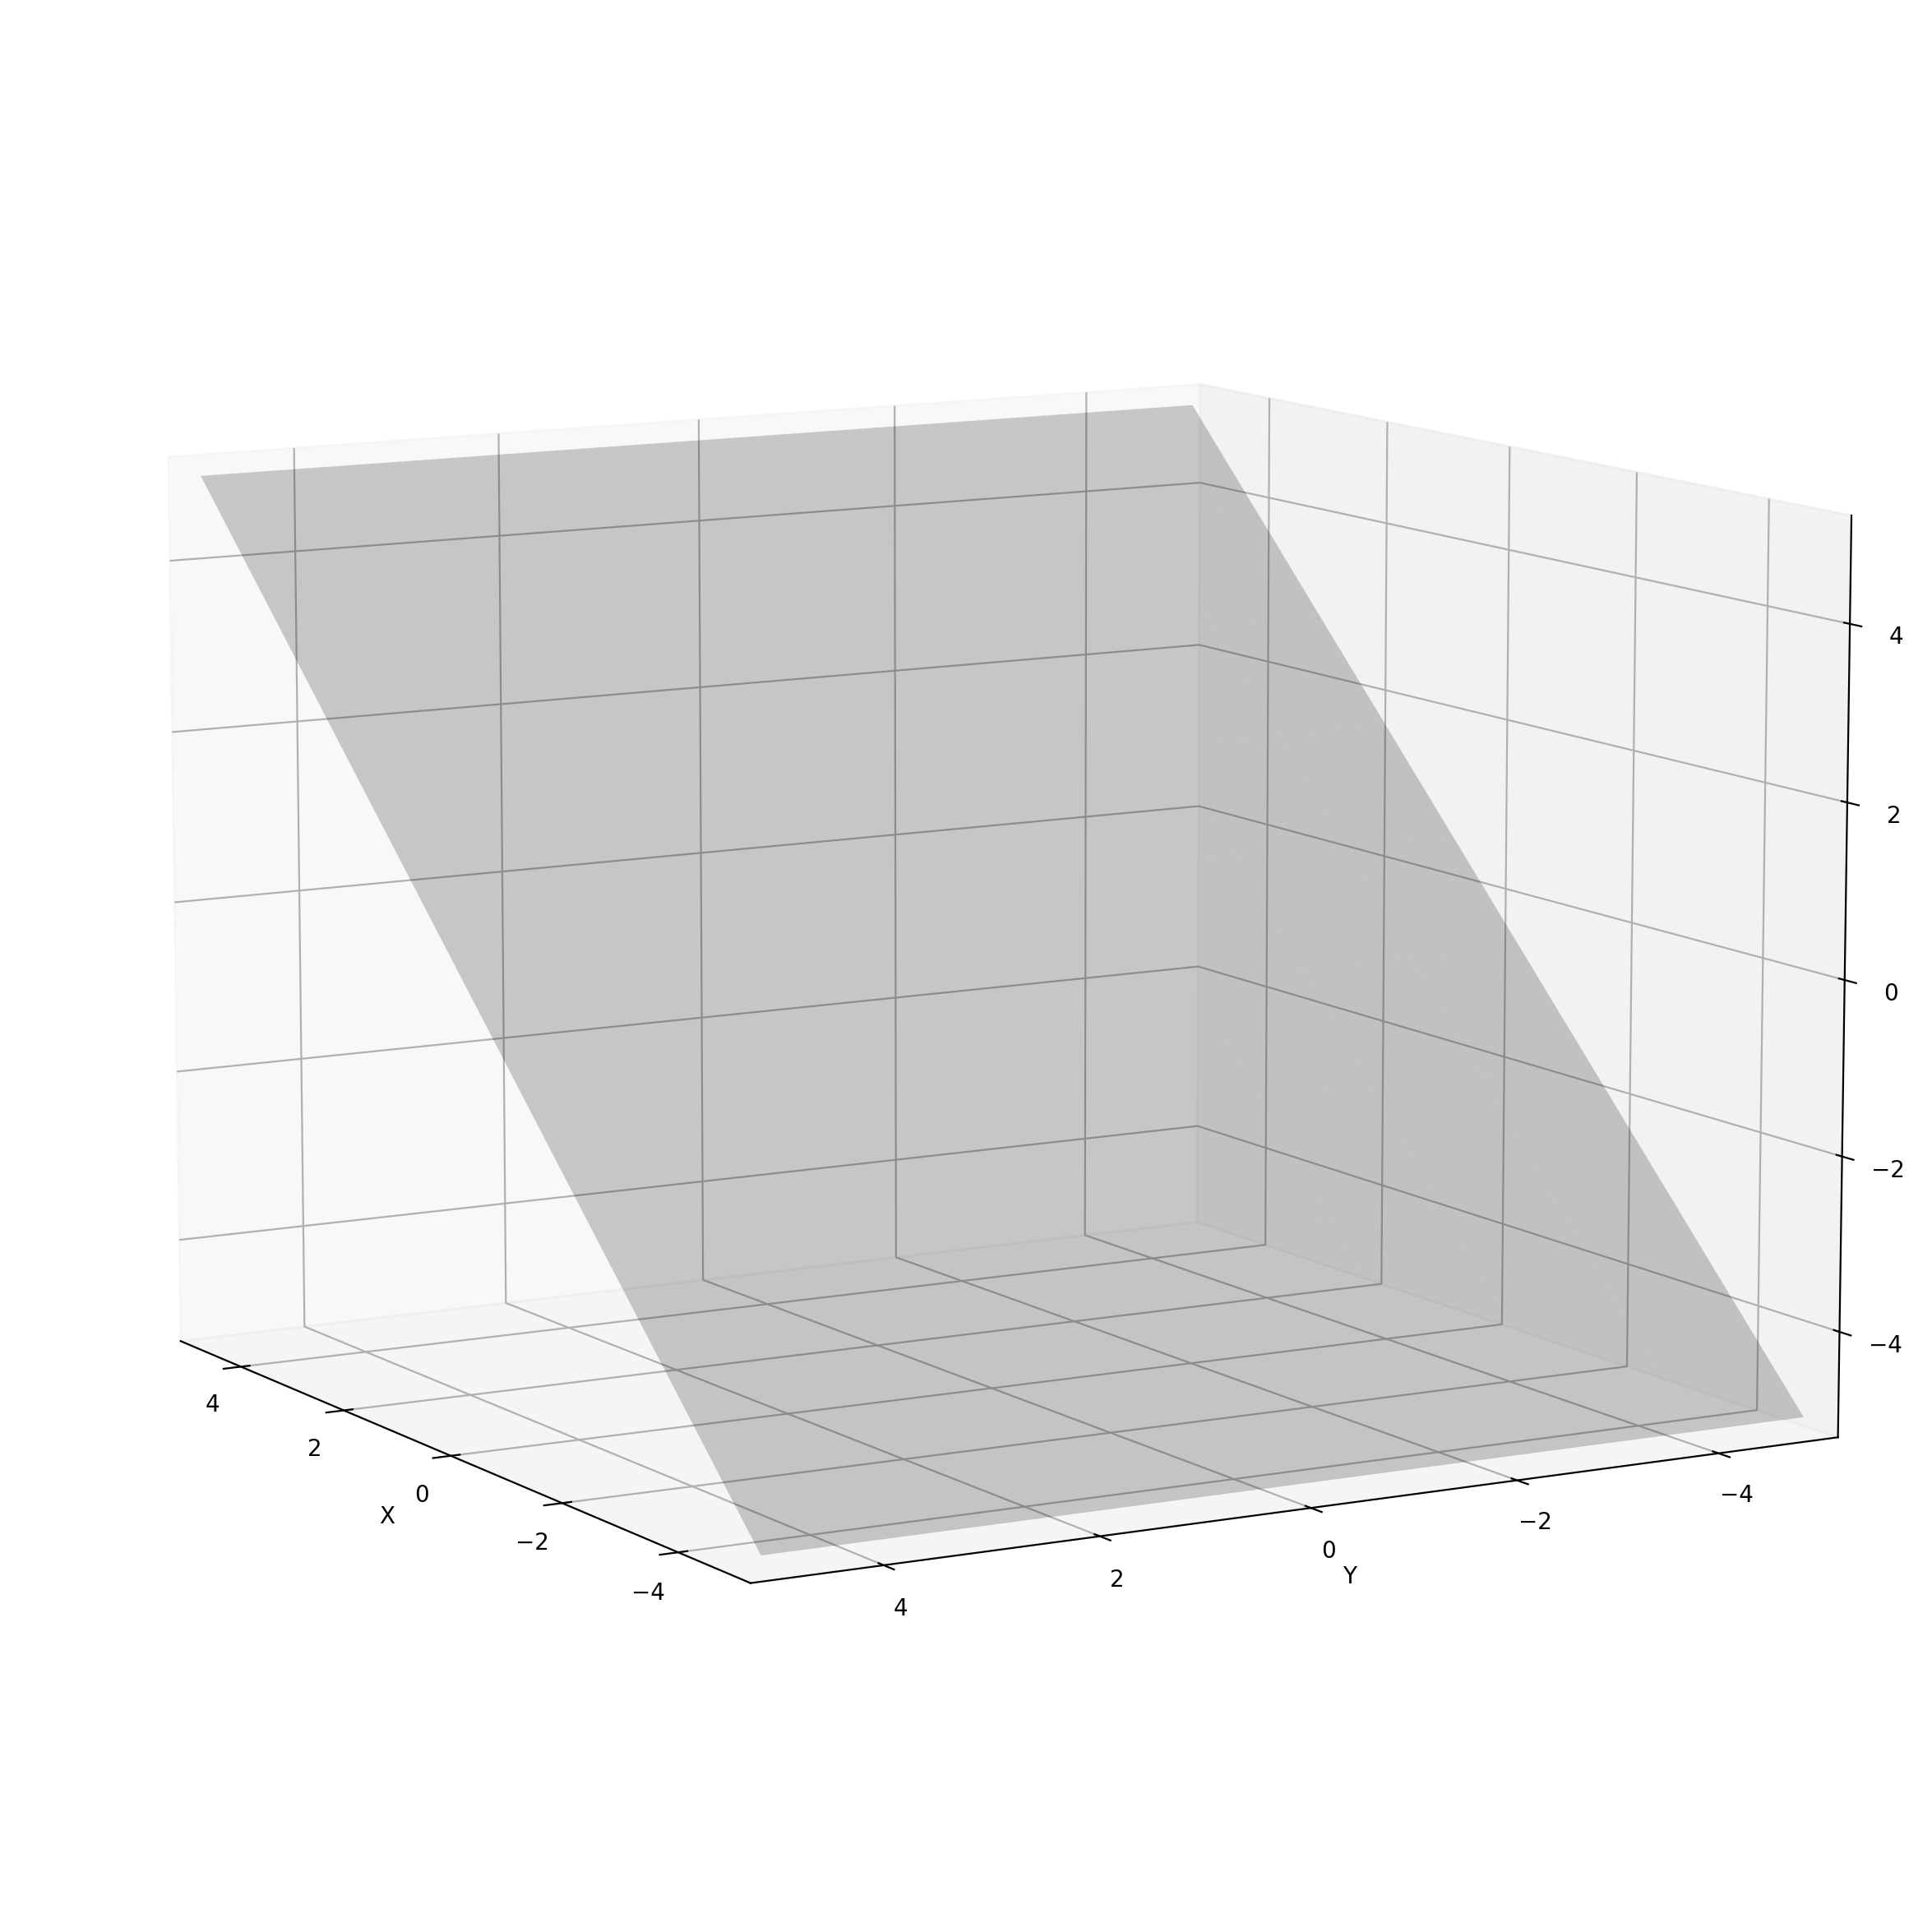
\includegraphics[scale=0.39]{Images/vector-space-ex.png}
    \caption{Graphical representation of $V$ vector space.}
    \label{fig:vector-space-ex}
\end{figure}

%%%%%%%%%%%%%%%%%%%%%%%%%%%%%%%%%%%%%%%%%%VECTOR-SUBSPACE%%%%%%%%%%%%%%%%%%%%%%%%%%%%%%%%%%%%%%%%%%%%%%%%%
\subsection{Vector Subspaces}

Let $V$ be a vector space over a field $\mathbb{F}$, and let $W$ be a non-empty subset of $V$. $W$ is called a \emph{vector subspace} of $V$ if it satisfies the following properties:

\begin{enumerate}
    \item \textbf{Closure under Vector Addition:} For any $\vec{u}, \vec{v} \in W$, their sum $\vec{u} + \vec{v}$ is also in $W$.
    
    \item \textbf{Closure under Scalar Multiplication:} For any $\vec{v} \in W$ and any scalar $c \in \mathbb{F}$, the scalar product $c\vec{v}$ is in $W$.
    
    \item \textbf{Contains the Zero Vector:} The zero vector $\vec{0}$ of $V$ is in $W$.
\end{enumerate}

If these conditions are met, $W$ is a vector subspace of $V$ and is denoted as $W \subseteq V$.
\\

\textbf{Example of Vector Subspace}

Consider \(W\) as a vector subspace of previously defined space \(V\):

$$
\scalebox{1.1}{$W \subseteq V = \{\vec v \in \mathbb{R}^3 \ | \ v_3 = v_1\}$}
$$$$
\scalebox{1.1}{$W = \{ \vec{w} \in \mathbb{R}^3 \mid w_3 = w_1 \land w_1 + w_2 = 0\}$}
$$

In other words, \(W\) consists of all vectors in \(\mathbb{R}^3\) whose component $w_3$ is equal to $w_1$ and $w_1$ and $w_2$ components sum to zero.
\\

Let's check the three conditions for \(W\) to be a vector subspace:

\begin{enumerate}
    \item \textbf{Closure under Addition:}
     \begin{itemize}
            \item Take \(\vec{v} =\begin{bmatrix} v_1 \\ -v_1 \\ v_1 \end{bmatrix}\) and \(\vec{w} =\begin{bmatrix} w_1 \\ -w_1 \\ w_1 \end{bmatrix}\) where \(\vec v, \vec w \in W \).
            \item Their sum \(\vec{v} + \vec{w} =\begin{bmatrix} v_1 + w_1 \\ -(v_1 + w_1) \\ v_1 + w_1 \end{bmatrix} = \vec z\) is also in \(W\) because \(z_2 = -z_1 \land z_3 = z_1\).
        \end{itemize}
        
    \item \textbf{Closure under Scalar Multiplication:}
     \begin{itemize}
            \item Take \(\vec{w} =\begin{bmatrix} w_1 \\ -w_1 \\ w_1 \end{bmatrix} \in W\) and \(k \in \mathbb{R}\).
            \item The scalar multiple \(k \cdot \vec{w} =\begin{bmatrix} kw_1 \\ -(kw_1) \\ kw_1 \end{bmatrix} = \vec z\) is also in \(W\) since \(z_1 = -z_2 \land z_3 = z_1\).
        \end{itemize}
    
    \item \textbf{Contains the Zero Vector:}
     \begin{itemize}
            \item The zero vector \(\vec{0} =\begin{bmatrix} 0 \\ 0 \end{bmatrix}\) is in \(W\) because \(z_1 = -z_2 \land z_3 = z_1\).
        \end{itemize}
\end{enumerate}
Therefore, \(W\) satisfies all conditions and is indeed a vector subspace of \(V\).
\\

The graphical representation of the vector subspace $W$ is a one-dimensional line as shown in Figure \ref{fig:vector-subspace-ex}.
\begin{figure}[h]
    \centering
    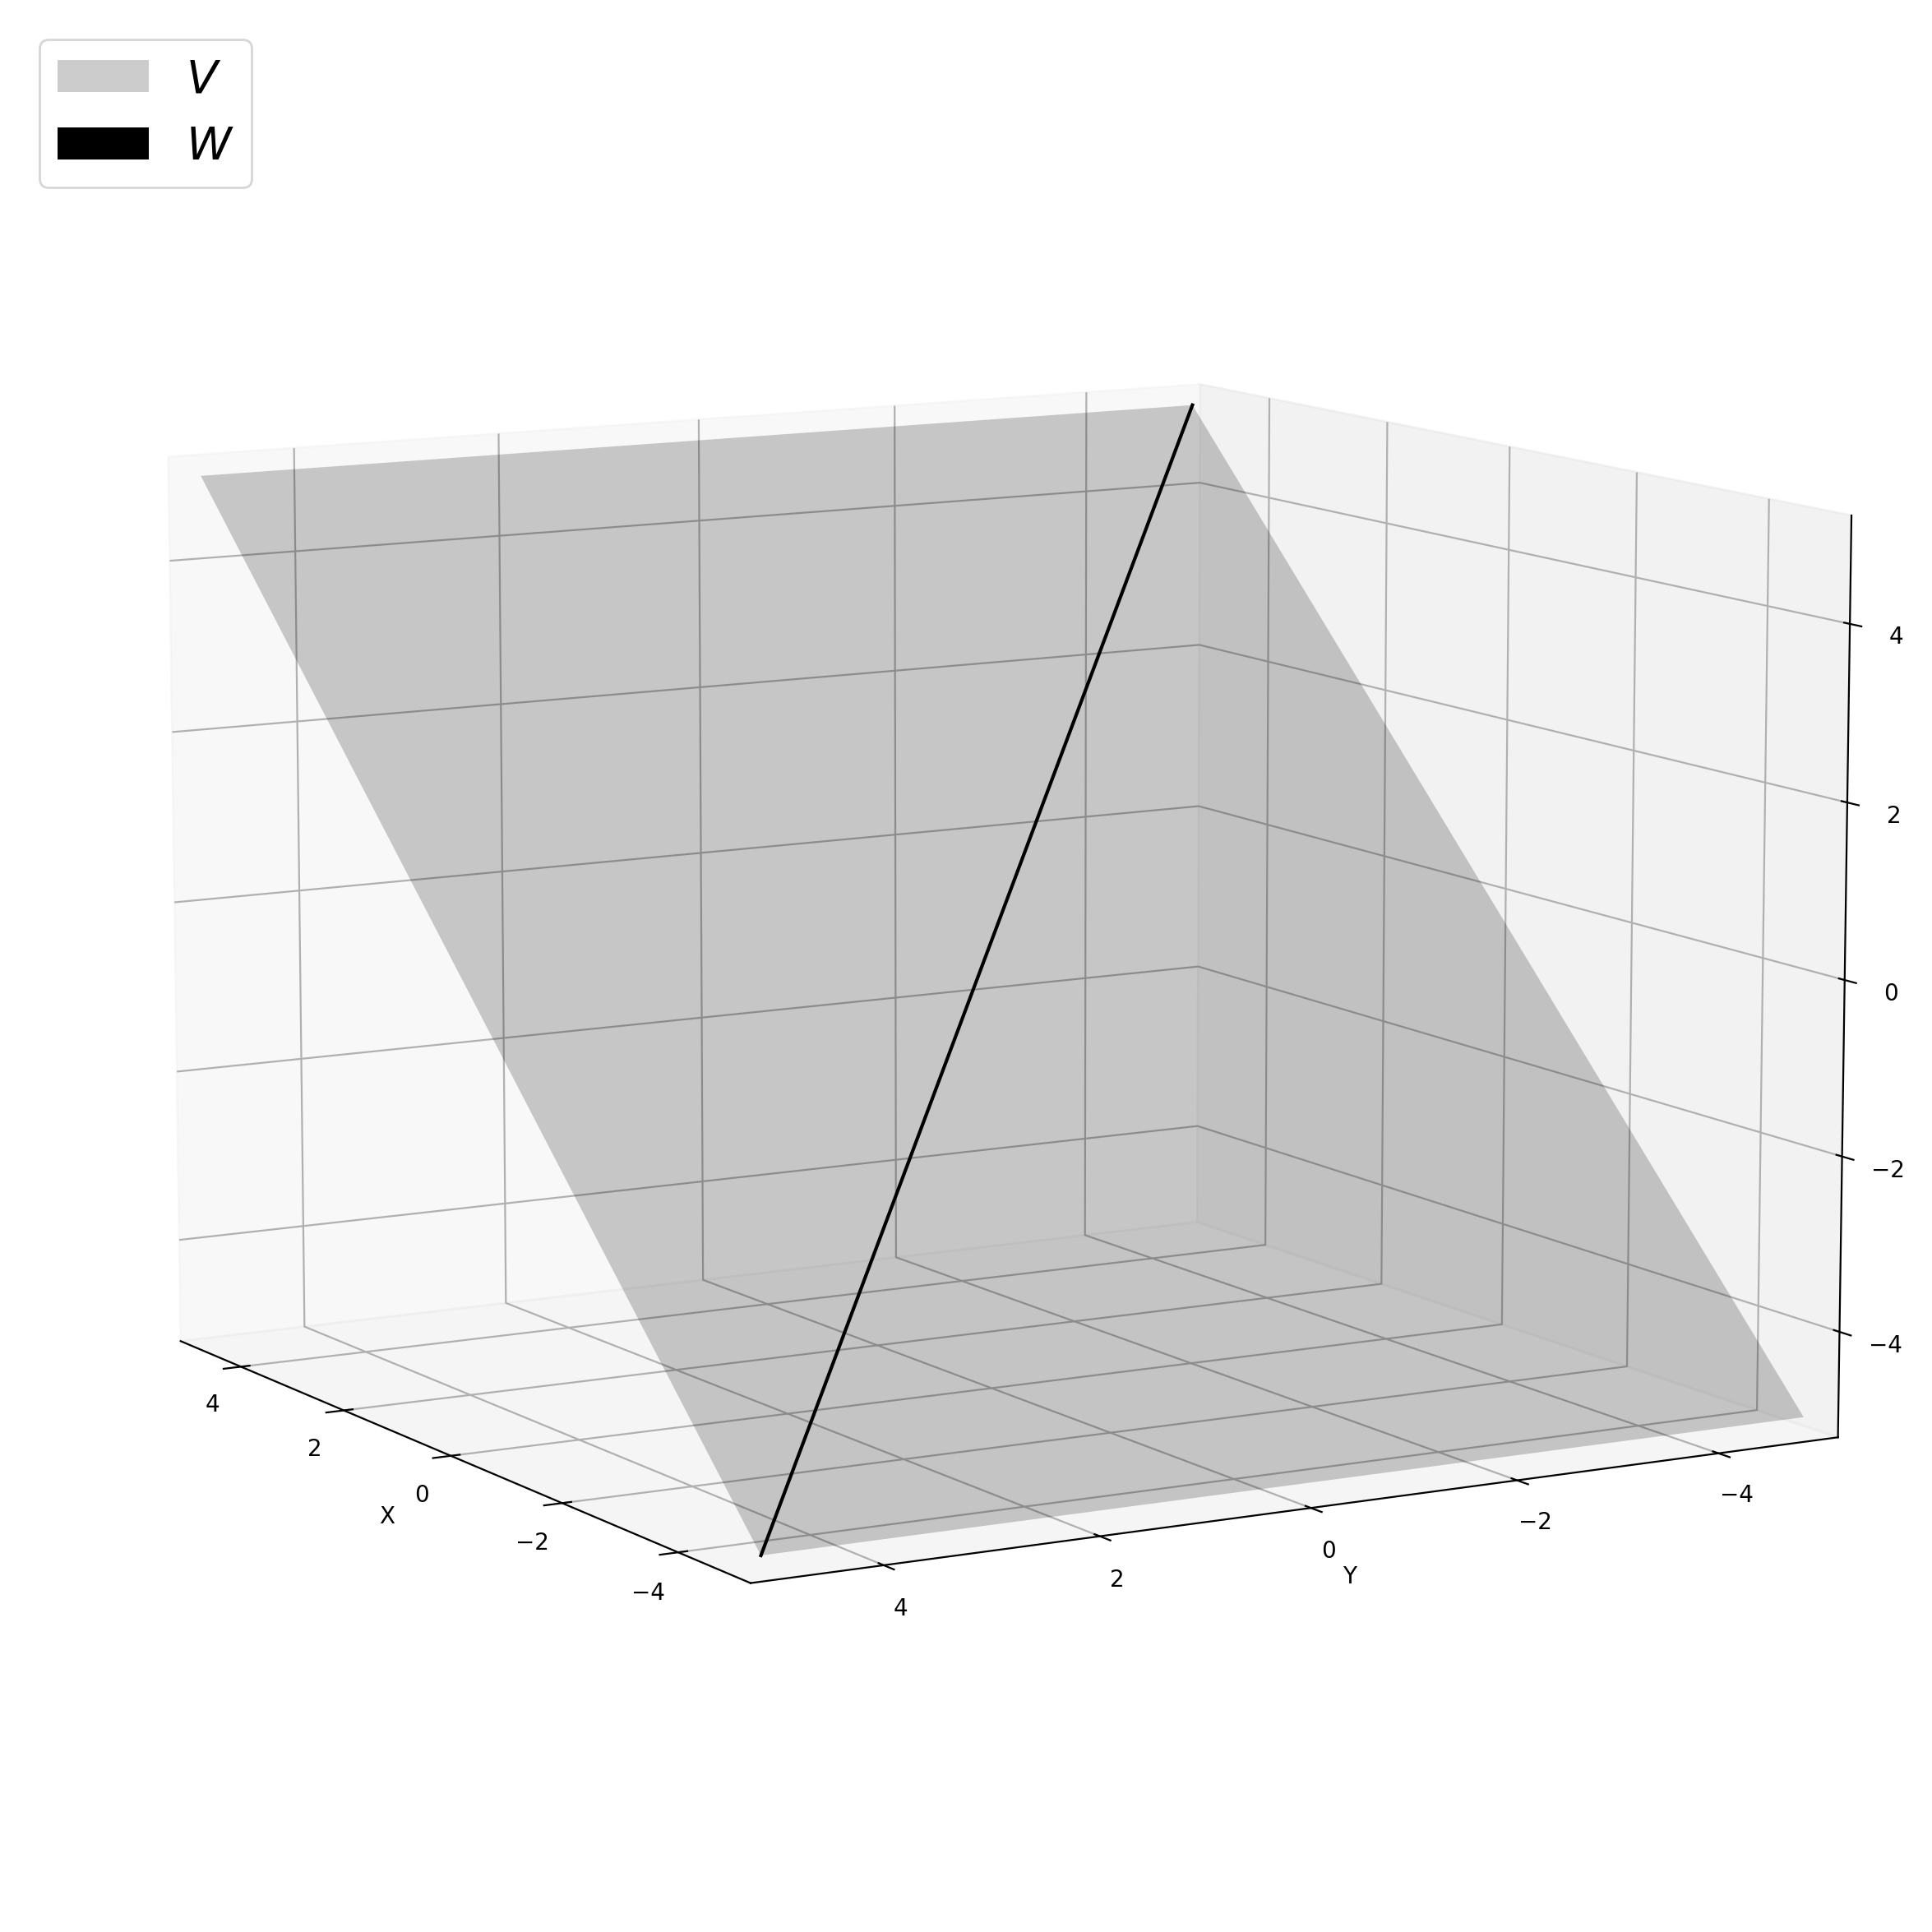
\includegraphics[scale=0.36]{Images/vector-subspace-ex.png}
    \caption{Graphical representation of $V$ vector space (gray) and $W$ vector subspace (black).}
    \label{fig:vector-subspace-ex}
\end{figure}

\subsubsection{Sum of Subspaces}

Let $U_1, \ldots, U_m$ be subspaces of $V$. The sum $U_1 + \cdots + U_m$ is a vector subspace of $V$, defined as the set of all possible sums of elements from $U_1, \ldots, U_m$, denoted by:

\[ U_1 + \cdots + U_m = \{ u_1 + \cdots + u_m : u_1 \in U_1, \cdots, u_m \in U_m \} \].

This sum represents the space formed by combining elements from each subspace. 
\\

The union of basis vectors (of each base) of each subspace is a spanning set for the new sum vector subspace $ U_1 + \cdots + U_m$.
\\

Note that if 

\begin{enumerate}
    \item $U_1 + \cdots + U_m = V$
    \item $U_1 \cap \cdots \cap U_m = \{\vec 0\}$
\end{enumerate}

The sum $U_1 + \cdots + U_m$ is called \textbf{direct sum} and it is denoted as

\[ U_1 \oplus \cdots \oplus U_m = \{ u_1 + \cdots + u_m : u_1 \in U_1, \ldots, u_m \in U_m\} \].

In a direct sum, every element of $U_1 \oplus \cdots \oplus U_m$ can be uniquely expressed as a sum $u_1 + \cdots + u_m$, where each $u_j$ belongs to $U_j$. And the only way to write 0 as a sum $u_1+...+u_m$ is by taking each $u_j$ equal to 0. So the union of the basis vectors (of each basis) of each vector space, form a basis for the new sum vector space.
\\

This represents a decomposition of the vector space $V$ into mutually exclusive subspaces, where each element has a unique representation as a sum of elements from the respective subspaces.
\\

%%%%%%%%%%%%%%%%%%%%%%%%%%%%%%%%%%%%%%%%Intersection-union%%%%%%%%%%%%%%%%%%%%%%%%%%%%%%%%%%%%%%%%%%%%
\subsubsection{Intersection of Subspaces}

Consider subspaces $V$ and $W$ of a vector space $U$. The intersection $V \cap W$ is also a subspace of $U$.

Since both $V$ and $W$ are subspaces, they contain the zero vector, making $V \cap W$ nonempty. Let $\vec v_1, \vec v_2 \in V \cap W$. As $V$ and $W$ are closed under addition, $\vec v_1 + \vec v_2 \in V$ and $\vec v_1 + \vec v_2 \in W$, implying $\vec v_1 + \vec v_2 \in V \cap W$. Thus, $V \cap W$ is closed under addition.

Consider $c \in \mathbb{R}$ and $v \in V \cap W$. Since $V$ and $W$ are closed under scalar multiplication, $c \vec v \in V$ and $c \vec v \in W$, indicating $c \vec v \in V \cap W$. Therefore, $V \cap W$ is closed under scalar multiplication.

These closures demonstrate that the intersection of subspaces preserves the subspace property within the overarching vector space $U$.

\subsubsection{Union of Subspaces}

In contrast, the union of subspaces $V$ and $W$ may not form a subspace of $U$. For instance, consider two distinct lines passing through the origin in $\mathbb{R}^2$. While each line individually forms a subspace, their union lacks closure under addition, failing to be a subspace.